% It doesn’t do anything, per se, it just warns when you accidentally
% use deprecated LaTeX constructs from l2tabu
\RequirePackage[l2tabu, orthodox]{nag}

%% THis is to resolve error 131 in adobe reader
%\pdfobjcompresslevel=1

%\pdfminorversion=4
% Check https://en.wikibooks.org/wiki/LaTeX/Document_Structure for
% more info
\documentclass[
a4paper,
12pt,
]{report}

%%%%%%%%%%%%%%%%%%%%%%%%%%%%%%%%%%%%%%%%%%%%%%%%%%%%%%%%%%%%%%%%%%%%%%%%%%%%%%%%
% Include packages
%%%%%%%%%%%%%%%%%%%%%%%%%%%%%%%%%%%%%%%%%%%%%%%%%%%%%%%%%%%%%%%%%%%%%%%%%%%%%%%%
% most of the packages bellow are from
% http://tex.stackexchange.com/questions/553/what-packages-do-people-load-by-default-in-latex

% less hyphens... (works only with pdflatex)
% stretch=10 allows font expansion up to 1% (default is 2%)
\usepackage[stretch=10]{microtype}
% disable ff and fi etc. ligatures
\DisableLigatures{encoding = *, family = *}
% allow breakable urls
\usepackage[hyphens]{url}
% If grouped citations are in the same order put the range i.e. 5-7
% DOES NOT WORK WITH biblatex package
%\usepackage{cite}
% For hyperlinks and more in the pdfs
\usepackage{hyperref}
\hypersetup{
  linktoc=all,
  bookmarks=false,           % show bookmarks bar?
  bookmarksopen,
  bookmarksnumbered,
  colorlinks = true,
%  linkcolor=black,           % color of interlinks
  citecolor=black,           % color of the citation links
%  urlcolor=black,            % the url color
  unicode=true,              % non-Latin characters in Acrobat’s bookmarks
  pdftoolbar=true,           % show Acrobat’s toolbar?
  pdfmenubar=true,           % show Acrobat’s menu?
  pdffitwindow=true,         % window fit to page when opened
  pdftitle={greenvm User's Manual},  % title
  pdfborder={ 0 0 0 },        % uBorder tin links
  pdfauthor = {Foivos S. Zakkak},
  pdfcreator = {Foivos S. Zakkak},
}
% handles spaces in commands (i.e. \newcommand{\test}[0]{Test\xspace},
% this way \test will be replaced by Test and a space *iff* needed)
\usepackage{xspace}
% For citations and bibliographies, biblatex is the package of my
% choice
\usepackage{biblatex}
% The booktabs package creates much nicer looking tables than the
% standard latex tables;
\usepackage{booktabs}
% the array package's ability to create custom columns is invaluable
% for formatting tabular material on a per-column basis.
\usepackage{array}
% For unicode files
\usepackage[utf8]{inputenc}
% For including figures, rotating or scaling text. I also use the
% \graphicspath command to specify a subfolder to help organize my
% figures and so I can easily change between, for example, a set of
% figures for internal used (with extra info) and final versions for
% distribution.
\usepackage{graphicx}
% define the default path for the figures
\graphicspath{{figs/}}
% This package provides very sophisticated facilities for reading and
% writing verbatim TeX code. Users can perform common tasks like
% changing font family and size, numbering lines, framing code
% examples, colouring text and conditionally processing text.
\usepackage{fancyvrb}

% Using listings
\usepackage{listings}
% Change the listing captions
% to use \begin{lstlisting}[label=some-code,caption=Some Code]
\usepackage{caption}
\DeclareCaptionFont{white}{\color{white}}
\DeclareCaptionFormat{listing}{\colorbox{MidnightBlue}{\parbox{.98\textwidth}{#1#2#3}}}
\captionsetup[lstlisting]{format=listing,labelfont=white,textfont=white}
\renewcommand{\lstlistingname}{Code}
\renewcommand\lstlistlistingname{List of Codes}
\def\lstlistingautorefname{Code }
% lstset
\lstset{
  language=C,
  basicstyle=\sffamily,
  columns=flexible,
  numbers=left,
%   numberstyle=\em\scriptsize,s
  showstringspaces=false,
  alsoletter={-},
  morekeywords={in,out,inout,pragma,task,wait,all,safe,scoop,input,output,start,finish},
  otherkeywords={INOUT,INPUT,SAFE,OUTPUT,START},
  literate={-}{-}1,
  numbersep=1em,
  xleftmargin=2.5em,
  xrightmargin=1em,
  escapeinside={@}{@},
  morecomment=[l][\bf\color{BrickRed}]{\#pragma\ scoop},
  commentstyle=\color{gray},
%   identifierstyle=\color{green},
%   backgroundcolor=\color{gray},
  keywordstyle=\bf\color{MidnightBlue},
  stringstyle=\color{OliveGreen},
}
% Allow different numbering styles in enumerate environment
\usepackage{enumerate}
% Change the margins
\usepackage[margin=3cm]{geometry}
\setlength{\marginparwidth}{2.5cm}
% Adds the \todo command which adds nice todo blocks to the document
\usepackage{todonotes}
% change the side for the todos
\reversemarginpar
% I much prefer no indentation and space between paragraphs
\usepackage[parfill]{parskip}
% Add fonts
\usepackage{comfortaa}
% use tikz
\usepackage{tikz}
% For quotations
\usepackage[
indentfirst=true,
font=itshape,
begintext=\textquotedblleft,
endtext=\textquotedblright,
]{quoting}
%%%%%%%%%%%%%%%%%%%%%%%%%%%%%%%%%%%%%%%%%%%%%%%%%%%%%%%%%%%%%%%%%%%%%%%%%%%%%%%%


%% Boxes for notes and caution messages
\usetikzlibrary{shapes,snakes}
\tikzstyle{notebox} = [draw=yellow, fill=yellow!10, very thick,
    rectangle, rounded corners, inner sep=10pt, inner ysep=15pt]
\tikzstyle{notetitle} =[draw=yellow, fill=white, text=black, very thick]

\newcommand{\notebox}[1]{
  \begin{tikzpicture}
    \node [notebox] (box){%
      \begin{minipage}{.95\linewidth}
        #1
      \end{minipage}
    };
    \node[notetitle, rounded corners, right=10pt] at (box.north west) {Note:};
  \end{tikzpicture}%
}

\tikzstyle{cautionbox} = [draw=red, fill=red!10, very thick,
    rectangle, rounded corners, inner sep=10pt, inner ysep=15pt]
\tikzstyle{cautiontitle} =[draw=red, fill=white, text=black, very thick]

\newcommand{\cautionbox}[1]{
  \begin{tikzpicture}
    \node [cautionbox] (box){%
      \begin{minipage}{.95\linewidth}
        #1
      \end{minipage}
    };
    \node[cautiontitle, rounded corners, right=10pt] at (box.north west) {\textbf{Caution:}};
  \end{tikzpicture}%
}

%%

\renewcommand{\FancyVerbFormatLine}[1]{%
  \$ #1}
\DefineVerbatimEnvironment{bash}{Verbatim}{
  fontsize=\footnotesize,
  frame=lines,
  framesep=3mm,
  label={\normalsize{Code}},
  labelposition=topline,
  commentchar=\#,
}

\definecolor{g}{HTML}{0E3B12}
\definecolor{v}{HTML}{003366}
\newcommand{\gvm}{{\fontfamily{fco}\selectfont\textbf{\color{g}green\color{v}vm}}\xspace}
\newcommand{\mblaze}{MicroBlaze\texttrademark\xspace}
\newcommand{\java}{Java\texttrademark\xspace}

% \title{greenvm User's Manual}
% \author{Foivos S. Zakkak}

\begin{document}

\begin{titlepage}
\begin{center}

\href{http://www.ics.forth.gr/carv/greenvm}{
\includegraphics[width=.5\linewidth]{greenvm}}\\
\LARGE User's Manual\\[0.5cm]
\large \today

\vfill


\includegraphics[width=.5\linewidth]{myrmigki_color}\\

\vfill

\large Author: \href{mailto:zakkak@ics.forth.gr}{\textit{Foivos S. Zakkak}}\\[1cm]

Foundation for Research and Technology - Hellas (FORTH)\\
Institute of Computer Science\\
N. Plastira 100\\
Vassilika Vouton, GR-700 13 Heraklion, Crete, Greece\\[0.5cm]

\end{center}

\end{titlepage}

% \maketitle

\pagenumbering{Roman}
\pagestyle{plain}
\listoftodos
\newpage
\tableofcontents
\newpage
% \phantomsection \label{listoffig}
% \addcontentsline{toc}{chapter}{List of Figures}
% \listoffigures
% \newpage
% \phantomsection \label{listoflst}
% \addcontentsline{toc}{chapter}{List of Codes}
% \lstlistoflistings
% \newpage
% \phantomsection \label{listoftb}
% \addcontentsline{toc}{chapter}{List of Tables}
% \listoftables
% \newpage
\thispagestyle{empty}
\pagenumbering{arabic}
\pagestyle{headings}

\chapter*{Introduction}

\gvm is a \java Virtual Machine that uses software shared memory to run
parallel \java programs on non cache-coherent architectures.

\chapter{Design}

\gvm is currently implemented to run on the Formic cube.

\section{Formic cube's architecture overview}

The Formic cube consists of 64
\href{http://www.formic-board.com/}{Formic Boards} with a total of 512
\href{http://www.xilinx.com/tools/microblaze.htm}{\mblaze} cores.

Each Formic board features:
\begin{itemize}
\item 8 \mblaze 32-bit RISC CPUs running at 10MHz.
\item 128MB of memory (400MHz DDR DRAM)
\end{itemize}

Each \mblaze core features:
\begin{itemize}
\item a private two-way 4-KB instruction L1 cache
\item a private two-way 8-KB data L1 cache
\item a private eight-way 256-KB L2 unified cache
\item a DMA engine, supporting 64 outstanding DMAs (32 incoming and 32 outgoing)
\item a 4-KB mailbox (messages can be of one or two words or even one cache-line)
\item 128 counters, that support atomic increment, decrement and read
  (but no fetch and add or compare and swap etc.)
\end{itemize}
%\subsection{\mblaze}

\subsection{Technical information}
The Formic board provides protection per 1MB pages.

To flush only parts of the private caches the programmer needs to
issue a DMA transfer from the cache to the local DRAM.

DMA transfers operate on cache line granularity.

In each DMA engine serialization happens only between incoming and
between outgoing requests (they are handled by two different queues).

\section{Memory Management}
The Formic cube's total memory is 8GB ($64\times128$MB). However the
\mblaze processor can address up to 4GB of memory (32-bit CPU). In our
design we take advantage of this feature and split the memory to two
segments. On each Formic Board, 64MB are dedicated to provide a slice
of the \java heap which is addressable and accessible from every core
on the system. The remaining 64MB are used as follows. We reserve 4MB
for the binary code (read-only). We reserve 1MB per core for the
JVM's and the \java's stacks. Finally we reserve 6.5MB per core for
caching objects from \textit{remote} \java heap slices.

\begin{figure}[!ht]
  \centering
  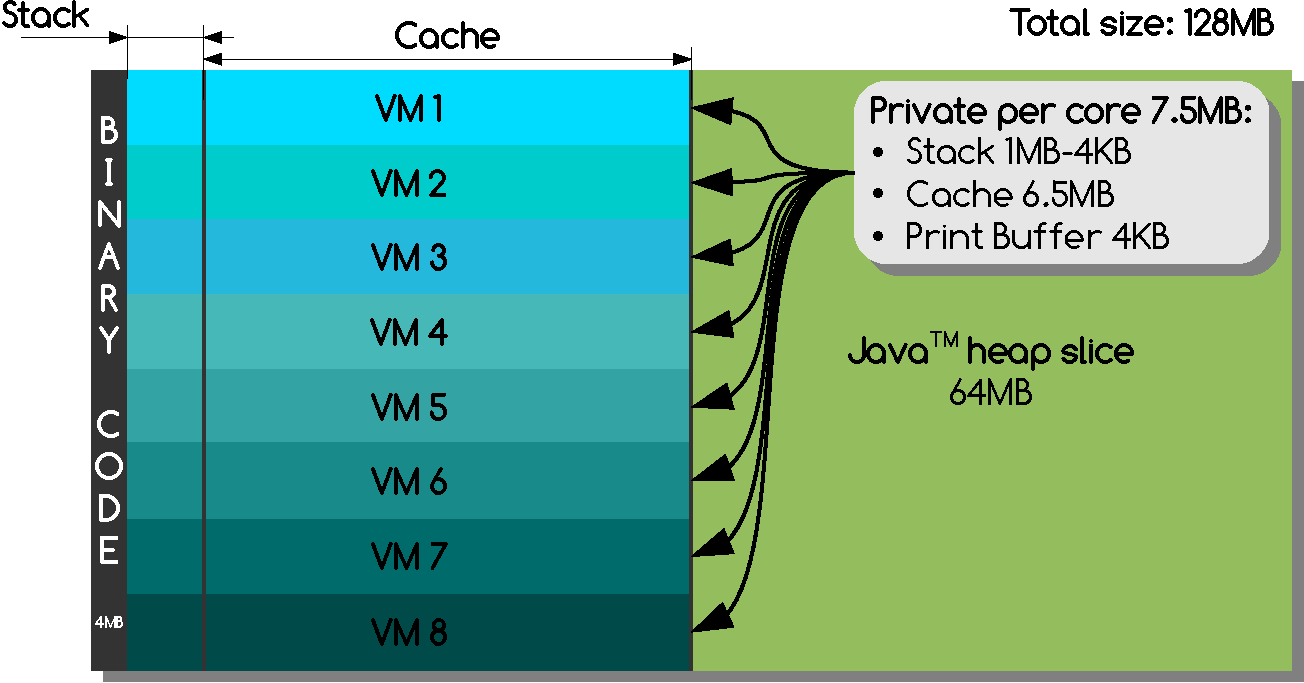
\includegraphics[width=\linewidth]{memmap}
  \caption{Memory Partitioning}
  \label{fig:memmap}
\end{figure}

\autoref{fig:memmap} is a visualization of the memory
partitioning. The dark block is the reserved space for the binary
code. The turquoise scales are the private memory segments used for
the JVM's and the \java's stacks as well as for caching. Each scale
denotes a different core. Finally the light green block is the memory
partition that serves as a heap slice.

Partitioning the \java Heap across 64 boards raises the need for
caching. To access an object that is located in a remote DRAM module a
DMA transfer for each access would be too expensive. To reduce the
overhead, \gvm is based on software caching at object granularity. In
case of arrays we use a block granularity (defined as a JVM argument).
Caching, however, requires extra effort in order to provide a coherent
view of the data, as it is defined by the \java Memory Model.

\subsubsection{The \java Memory Model}
Here, let us quote Jeremy Manson to give an informal and brief
description of the \java Memory Model:

\begin{quoting}
  1) Each thread in Java takes place in a separate memory space
  (this is clearly untrue, so bear with me on this one).\\
  \ ~2) You need to use special mechanisms to guarantee that
  communication happens between these threads, as you would on a
  message passing system.\\
  \ ~3) Memory writes that happen in one thread can ``leak through'' and
  be seen by another thread, but this is by no means
  guaranteed. Without explicit communication, you can't guarantee
  which writes get seen by other threads, or even the order in which
  they get seen.
\end{quoting}
Source: \url{http://jeremymanson.blogspot.com/2008/11/what-volatile-means-in-java.html}

According to the \java Memory Model. \java has the following
synchronization points.

\begin{itemize}
\item \verb!monitorenter!
\item \verb!monitorexit!
\item \verb!volatile! load
\item \verb!volatile! store
\item \verb!Thread.start()!
\item \verb!Thread.join()!
\item \verb!class! initialization (Constructors)
\item \verb!final! fields initialization
\end{itemize}

\notebox{
  Suggested reading material:
  \begin{itemize}
  \item \href{http://gee.cs.oswego.edu/dl/jmm/cookbook.html}{The JSR-133
      Cookbook for Compiler Writers}
  \item
    \href{http://www.cs.umd.edu/~pugh/java/memoryModel/jsr133.pdf}{JSR-133
      \java Memory Model and Thread Specification}
  \item
    \href{https://dl.dropboxusercontent.com/u/1011627/journal.pdf}{SPECIAL
      POPL ISSUE: The \java Memory Model}
  \end{itemize}
}

\subsection{Software Caching}
\label{sec:software-caching}

To implement the software caching with respect to the \java Memory
Model we have to satisfy the following conditions:

\begin{itemize}
\item Before each \verb!monitorenter!
  \begin{itemize}
  \item any preceding \verb!monitorexit!, \verb!monitorenter!,
    \verb!volatile! read or \verb!volatile! store must reach
    completion
  \item any preceding \verb!volatile! store's effects must become
    visible to the home node
  \item any preceding \verb!monitorexit!'s effects must become visible
    to the other cores/processors
  \item any outstanding write-backs from synchronization points must
    reach completion

    \notebox{The previous bullets are implicitly satisfied by the
      conditions of \texttt{monitorexit}, \texttt{volatile} store and
      \texttt{volatile} read that follow and the fact that \mblaze is
      \textit{inorder}}
  \end{itemize}
\item Before each \verb!monitorenter! completion
  \begin{itemize}
  \item Any cached objects must be updated (if there are newer
    versions at the home node available)

    \notebox{ The simplest way to achieve this, is to empty our
      software-cache and re-fetch the objects upon request.}

    \notebox{ Pre-fetching data would save a significant amount of
      time as the DMA transfers would overlap with code
      execution. However, for \gvm to be aware of what objects need to
      be fetched a priori, the programmer or even better a static
      analysis must provide appropriate hints. In a data-flow
      execution model this is even easier to achieve, combining the
      programmer's data-flow annotations with a static analysis on the
      code.}

    \notebox{ A possible improvement here would be to use versioning
      of the cached objects instead of flushing the whole software
      cache at every synchronization point. With versioning a core can
      simply query the \emph{home} DRAM for the latest version of the
      cached objects. Then it can only fetch the remote objects that
      feature a higher version number than the cached data. In this
      case we would probably like to use some dedicated cores (like
      the ones discussed in the next section) that would be
      responsible for answering such queries and even initiate the DMA
      transfers. The version number could be kept in the object's
      header.}
  \item the effects of this instruction (lock acquisition) must become
    visible to every core
  \end{itemize}

\item Before each \verb!monitorexit!
  \begin{itemize}
  \item any preceding load or store must complete

    \notebox{This is implicitly satisfied by the \texttt{volatile}
      store completion conditions that follow and the fact that
      \mblaze is \textit{inorder}}
  \item any preceding \verb!monitorenter! or \verb!monitorexit!
    instruction must reach completion
  \end{itemize}
\item Before each \verb!monitorexit! completion
  \begin{itemize}
  \item all \emph{dirty} objects (on this core) must get written-back
    to the memory

    \notebox{ There is no need to empty our software-cache. }

    \notebox{ Here it is not mandatory to block until the write-back
      reach completion. However to do this we need a mechanism to
      notify the home node that there are pending write-backs so
      potential readers will block until completion of the DMA
      transfers. Furthermore it would break the implicit satisfaction
      of some of the \textit{monitorenter} and \texttt{volatile} load
      bullets. }
  \end{itemize}

\item Before each \verb!volatile! store or \verb!volatile! read
  \begin{itemize}
  \item any preceding load or store must complete

    \notebox{This is implicitly satisfied by the \texttt{volatile}
      store completion conditions that follow and the fact that
      \mblaze is \textit{inorder}}
  \item any preceding \verb!monitorexit! or \verb!monitorenter!
    !instructions must reach completion
  \item any outstanding write-backs from synchronization points must
    reach completion
  \item Any cached objects must be updated (if there are newer
    versions at the home node available)

    \notebox{Look at \texttt{monitorenter} conditions for some notes
      on this}
  \end{itemize}
\item Before each \verb!volatile! store completion
  \begin{itemize}
  \item all \emph{dirty} objects (on this core) must get written-back
    to the memory

    \notebox{ There is no need to empty our software-cache. }

    \notebox{ Here it is not mandatory to block until the write-back
      reach completion. However to do this we need a mechanism to
      notify the home node that there are pending write-backs so
      potential readers will block until completion of the DMA
      transfers. Furthermore it would break the implicit satisfaction
      of some of the \textit{monitorenter} and \texttt{volatile} load
      bullets. }
  \item the effects of this instruction must be written-back to the
    home node
  \end{itemize}

  \notebox{ One might note that the effects of a \texttt{volatile}
    store are almost identical to that of \texttt{monitorexit}}
\item Before each \verb!volatile! read completion
  \begin{itemize}
  \item all \emph{dirty} objects (on this core) must get written-back
    to the memory

    \notebox{ There is no need to empty our software-cache. }

    \notebox{ Here it is not mandatory to block until the write-back
      reach completion. However to do this we need a mechanism to
      notify the home node that there are pending write-backs so
      potential readers will block until completion of the DMA
      transfers. Furthermore it would break the implicit satisfaction
      of some of the \textit{monitorenter} and \texttt{volatile} load
      bullets. }
  \end{itemize}

\item After the completion of a \verb!Thread.start()! call the newly
  created thread must be able to see the same stores its creator was
  able to see at the calling point.

  \notebox{
    A simple approach is to write-back \emph{dirty} objects and let the
    newly created thread fetch them if it needs them.
  }

  \notebox{
    Another approach is to copy the software-cache state of the
    caller core to the core where the newly created thread is going
    to be executed. This, however, is not straightforward when there
    are more \java threads than cores. Furthermore, before the copy
    we must ensure that any dirty data from the hardware-cache are
    written-back to the software-cache.
  }

\item After the completion of a \verb!Thread.join()! call the calling
  thread must be able to see the same stores the terminating thread
  was able to see.

  \notebox{
    This case is trickier than the
    previous. In this case we have two different live threads and we
    need to merge their software-caches. By simply copying the
    terminating thread's software-cache to the caller we could loose
    changes made by the caller thread, which is undesirable.
    A simple implementation would be to write-back any
    \emph{dirty} objects from the caller's software-cache and then
    copy over the terminating thread's software-cache. A more
    efficient approach would be to implement a mechanism for
    software-cache merging. The mechanism needs to identify which
    cached objects correspond to the same heap object and then keep
    the terminating thread's copy, updating the bookkeeping
    data-structures as needed.
  }
\item All \verb!static final! fields must be initialized before the
  object can be accessed.

\item Before using any object instance we have to make sure its
  initialization reached completion.

  \notebox{ Squawk should already be taking care of the previous two
    bullets. If not, a simple solution is to use a ready flag per
    object (probably in its header).}
\end{itemize}

\cautionbox{ JNI routine's entry and exit points are not
  synchronized. It is the programmer's responsibility to ensure her
  native code does not break the \java Memory Model semantincs.}

\section{Locks/Monitors}

In \java, each object reference can be used as a lock. In most \java
Virtual Machines this implies one extra field per object that is used
as a lock. In our design we decouple the locks from the objects but
still respect the tight relation between them. We use dedicated cores
for the lock management (less than one per board). When the virtual
machine executes a \verb!monitorenter! or a \verb!monitorexit!
bytecode it sends an appropriate message to the \emph{lock manager}
core responsible for the object reference passed as the bytecode's
argument. It's the \emph{lock manager} responsibility to handle this
request and reply appropriately to the \emph{sender}.

There are two possible scenarios when the virtual machine wants to
acquire a lock.
\begin{enumerate}[a)]
\item \textbf{The lock is free:} In this case the process is straight
  forward.  The \emph{lock manager} marks the lock as acquired and
  sends an acknowledgment message to the \emph{sender}.
\item \textbf{The lock is already taken:} In this case the \emph{lock
    manager} should reply with a negative acknowledgment. As a first
  approach the \emph{sender} should keep requesting to acquire the
  lock until it succeeds. Later on, we could allow the execution of
  other threads/tasks between the requests.
\end{enumerate}

With each object's lock being handled by one single core, we can
ensure that there is no possibility for two different \java threads to
enter the same critical region concurrently. The \emph{lock manager's}
mailbox acts as a serialization point for the acquire and release
requests.

\chapter{Implementation}
\label{cha:implementation}

\section{Choosing the code base}

At the early stages we examined the following list of \java virtual
machines.

\begin{itemize}
\item Squawk
  \begin{itemize}
  \item Still active
  \item ~150k LOC of which 8k are C and 590 are Assembly
  \item bare metal ready
  \end{itemize}
\item JamVM
  \begin{itemize}
  \item Last release Jan '10
  \item written for embedded
  \item mostly interpreter
  \item small footprint
  \item well structured
  \item 19391 LOC
  \end{itemize}
\item hotspot
  \begin{itemize}
  \item the official
  \item complex
  \item posix
  \item JIT and Interpreter
  \item ~450000 LOC
  \end{itemize}
\item kaffe
  \begin{itemize}
  \item Well known
  \item Inactive for many years
  \item 64376 LOC
  \end{itemize}
\item CACAO
  \begin{itemize}
  \item Last release Sept '12
  \item JIT
  \item Used to be the default for OpenJDK
  \item Well documented
  \item 121175 LOC
  \end{itemize}
\item sableVM
  \begin{itemize}
  \item Claims to be "A robust, clean, easy to maintain and extend,
     extremely portable, efficient, and specification-compliant Java
     virtual machine."
  \item 3 flavors of threaded interpretation (switched, threaded and
     inlined),
  \item bidirectional object layout,
  \item spinlock-free thin locks,
  \item sparse interface vtables,
  \item low-cost maps for precise garbage collection.
  \item limited by the current state of the class libraries, and
    occasionally lacks VM support for some class library features.
  \item 216893 LOC
  \end{itemize}
\item llvm-vmkit
  \begin{itemize}
  \item depends on llvm for JIT
  \item complex and big
  \end{itemize}
\item jikesrvm
  \begin{itemize}
  \item java source
  \item ant build system
  \item requires another JVM to run it
  \end{itemize}
\item gcj
  \begin{itemize}
  \item complex source code
  \item no VM
  \end{itemize}
\end{itemize}


We finally decided to build \gvm on top of
\href{https://java.net/projects/squawk/pages/SquawkDevelopment}{Squawk}.
This decision was mostly driven by the fact that Squawk was the only
\java virtual machine that was able to run on bare metal.  Squawk is a
good quality \java virtual machine that was used commercially on the
\href{http://www.sunspotworld.com/}{Sun Spot} platform.  Squawk comes
only with an interpreter and no JIT (Just-In-Time compilation) support.

\section{Squawk's specification overview}
\todo{write down the most important things from
  \href{http://java.net/projects/squawk/sources/svn/content/trunk/doc/TheSquawkSystem-Sep02.pdf}{here}
  plus personal experiences}

\section{\gvm limitations}

Squawk is designed to support the
\href{https://en.wikipedia.org/wiki/CLDC}{Connected Limited Device
  Configuration (CLDC)} 1.1.  CLDC is designed to work with \java 1.4
which is considered outdated.  We modified Squawk's toolchain to use
\href{http://retrotranslator.sourceforge.net/}{retrotranslator} to be
able to compile 1.5 source code to valid 1.4 classes.  This way we are
able to run \java 1.5 applications.

However, there are still some limitations that we did not put effort
to overcome.

\begin{itemize}
\item \verb!java.lang.reflect! is entirely missing, leaving us without
  reflection
\item We don't support finalization. CLDC does not include the
  Object.finalize() method
\item Many JavaSE 1.5 libraries are missing
\item No I/O is supported except from printing
\item Float autoboxing in throwException (breaks preverify)
\item errno is \textbf{NOT} implemented

\end{itemize}
% FIXME: might be more, but those are known ATM.

\section{Garbage Collection}

Currently there are three garbage collectors available in Squawk.

\begin{itemize}
\item \href{https://en.wikipedia.org/wiki/Cheney%27s_algorithm}{Cheney} (semispace)
\item Lisp2
\item Lisp2Generational
\end{itemize}

Non of this garbage collectors is suitable for \gvm though. That said,
\gvm needs to implement its own garbage collector. \todo{work package:
  GC}

\chapter{Configure, Build, Deploy}

\section{Dependencies}

In order to build \gvm you will need:

\begin{itemize}
\item Xilinix Tools (only for deploying on the Formic board: see
  \autoref{sec:xilinx-tools})
\item JDK 1.5 or later
\item git
\item GNU make
\item awk
\item sed
\item wc (wordcount)
\item od (objectdump)
\end{itemize}

\section{Build}

\subsection{On Formic Board (Microblaze)}
build-mb.properties contains the configuration of the microblaze
builds.

To create all needed files execute:
\begin{bash}
make -f mb.mk
\end{bash}


To deploy on the Formic cube:
\begin{bash}
make -f mb.mk run
\end{bash}

\notebox{ Your IP must be allowed to access formicarium. Please
  contact \href{mailto:zakkak@ics.forth.gr}{zakkak@ics.forth.gr} if
  your IP is not whitelisted }

\cautionbox{
  When running on formicarium always \texttt{tail}
  /home/lyberis/measure.log and /home/lyberis/server.log to monitor
  the logs and make sure the cube shuts down when you finish.
}

\subsection{on X86}
build-x86.properties contains the configuration of the x86 builds

To build (the JVM) and run the current application execute

\begin{bash}
make -f x86.mk
\end{bash}

\subsection{Options}
To change the application you want to build define \verb!APP!. For
example

\begin{bash}
make -f mb.mk "APP=../formic-tests/HelloWorld"
make -f mb.mk "APP=../formic-tests/HelloWorld" run
\end{bash}

To change the Garbage collector you have to modify the
build.properties file \textbf{and} build-*.properties file of the
architecture you want to target.

\section{Romizing programs (a.k.a. creating *.suite files)}

First compile the *.java files as usual. Then using retrotranslator
transform them to 1.4 classes. Next, preverify them using the
preverify tool. Finally, invoke the romizer (through the builder) to
produce the final suite file out of the *.class files.

\section{Xilinx Tools}
\label{sec:xilinx-tools}

\paragraph{Download and extract:}
\href{http://www.xilinx.com/support/download/index.html/content/xilinx/en/downloadNav/design-tools/v12_4.html)}
{ISE  Design Suite - 12.4 Full Product Installation}

\begin{bash}
tar xvf Xilinx_ISE_DS_Lin_12.4_M.81d.2.0.tar
\end{bash}

\paragraph{Install:}
\begin{bash}
sudo ./xsetup
\end{bash}

\paragraph{License:} 27000@carvouno.ics.forth.gr

\paragraph{Scripts to source:}
\begin{bash}
. /opt/Xilinx/12.4/ISE_DS/EDK/settings64.sh /opt/Xilinx/12.4/ISE_DS/EDK
. /opt/Xilinx/12.4/ISE_DS/ISE/settings64.sh /opt/Xilinx/12.4/ISE_DS/ISE
#. /opt/Xilinx/12.4/ISE_DS/PlanAhead/settings64.sh /opt/Xilinx/12.4/ISE_DS/PlanAhead
. /opt/Xilinx/12.4/ISE_DS/common/settings64.sh /opt/Xilinx/12.4/ISE_DS/common
\end{bash}

It is recommended to avoid adding these lines in your .bash\_profile or
.bashrc

\paragraph{For the usb JTAG programmer:}
If you are planning to deploy on a Formic Board using your usb port
you will need to follow
\href{http://www.george-smart.co.uk/wiki/Xilinx_JTAG_Linux}{this}
tutorial.


In case it fails try the following alternatives:
\begin{itemize}
\item \url{http://www.petalogix.com/support/kb/xilinx_ubuntu_install}
\item \url{http://forums.xilinx.com/t5/Installation-and-Licensing/installing-platform-cable-USB-II-ubuntu/td-p/66729}
\item \url{http://rmdir.de/~michael/xilinx/}
\end{itemize}
\end{document}
